\chapter{Лабораторная работа №1\\
Исследование влияния разброса параметров фильтра на АЧХ фильтра
}

\section{Пример}

Соберём фильтр нижних частот, изображённый на рис.~\ref{fig:example_schematic}.

Частота среза фильтра равна $550~\text{МГц}$, а уровень сигнала в полосе пропускания должен быть не меньше $3~\text{дБ}$.
Компоненты фильтра имеет следующие параметры:
\begin{itemize}
    \item $L_1 = L_4 = 15~\text{нГн}$;
    \item $L_2 = L_3 = 30~\text{нГн}$;
    \item $C_1 = C_3 = 8~\text{пФ}$;
    \item $C_2 = 10~\text{пФ}$;
\end{itemize}

\begin{figure}[!ht]
    \centering
    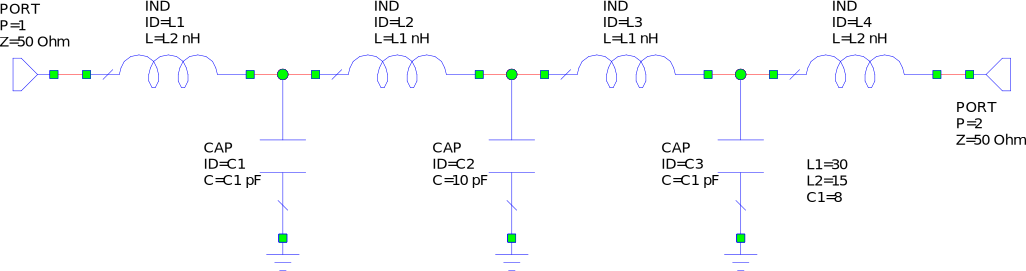
\includegraphics[width=0.8\textwidth]{example_schematic}
    \caption{Моделируемая схема}%
    \label{fig:example_schematic}
\end{figure}

При проведении статистического анализа установим изменение $L_2$ и $L_3$ в пределах $(20 \dots 40)~\text{нГн}$, $L_1$ и $L_4$ в пределах $(10 \dots 20)~\text{нФ}$, $C_1$ и $C_3$ в пределах $(6 \dots 10)~\text{пФ}$.
Частотный диапазон анализа --- $(0 \dots 1)~\text{ГГц}$ с шагом $0.02~\text{ГГц}$.

Результаты моделирования можно увидеть на рис.~\ref{fig:example_S21_yield_markers}.
Синей линией обозначена АЧХ, соответствующая основным номиналам компонентов, а серые соответствуют максимальному отклонению АЧХ при изменении номиналов в заданных пределах.

\begin{figure}[!ht]
    \centering
    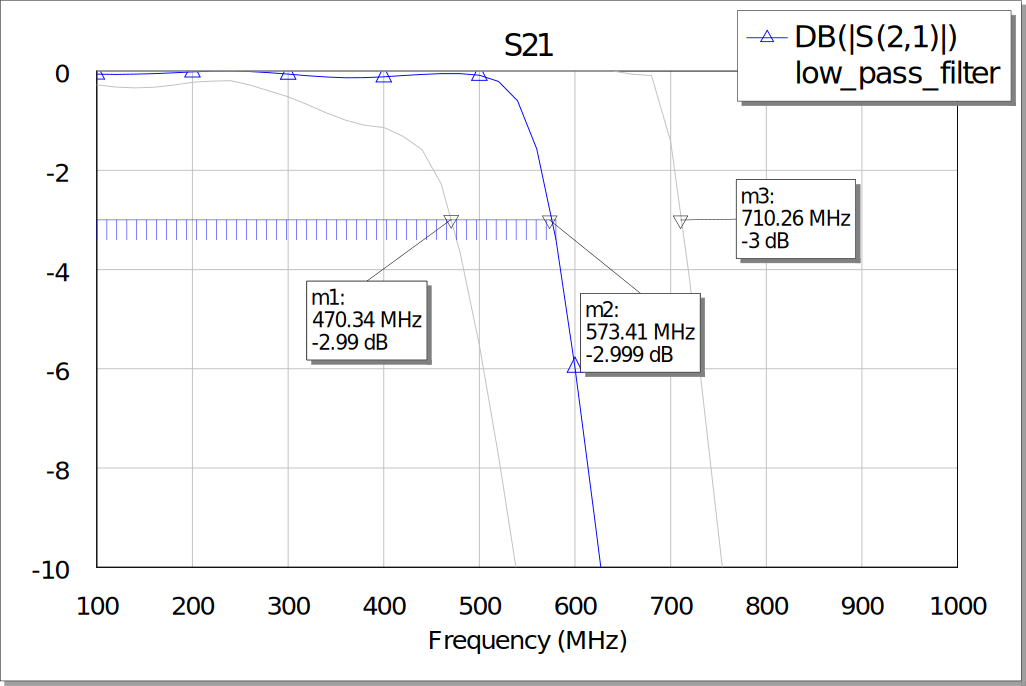
\includegraphics[width=0.8\textwidth]{example_S21_yield_markers}
    \caption{АЧХ проектируемого фильтра нижних частот}%
    \label{fig:example_S21_yield_markers}
\end{figure}

Из рисунка можно сделать вывод, что при точном соответвии номиналов установленным значениям, АЧХ фильтра удовлетворяет техническому заданию, но при заданном выше разбросе АЧХ может не удовлетворять техническому заданию.
Для того, чтоб исправить это, можно предпринять следующие действия: увеличить порядок фильтра, изменить номиналы компонентов.

\section{Вариант 2}

Спроектировать фильтр нижних частот со следующими параметрами: $L_1 = L_2 = L_3 = L_4 = 5~\text{нГн}$, $C_1 = C_3 = 5~\text{пФ}$, $C_2 = 10~\text{пФ}$, $f_{HPBW} = 1.5~\text{ГГц}$.

Схема моделируемого фильтра приведена на рис.~\ref{fig:task_schematic}.

\begin{figure}[!ht]
    \centering
    \includegraphics[width=\textwidth]{task_schematic}
    \caption{Моделируемая схема}%
    \label{fig:task_schematic}
\end{figure}

При проведении статистического анализа установим изменение $L_1$, $L_2$, $L_3$ и $L_4$ в пределах $(4.5 \dots 5.5)~\text{нГн}$, $C_1$ и $C_3$ в пределах $(4.5 \dots 5.5)~\text{пФ}$.
Частотный диапазон анализа --- $(0 \dots 2)~\text{ГГц}$ с шагом $0.02~\text{ГГц}$.

Результаты моделирования можно увидеть на рис.~\ref{fig:example_S21_yield_markers}.
Синей линией обозначена АЧХ, соответствующая основным номиналам компонентов, а серые соответствуют максимальному отклонению АЧХ при изменении номиналов в заданных пределах.

Из рисунка можно сделать вывод, что при точном соответвии номиналов установленным значениям, АЧХ фильтра не удовлетворяет техническому заданию, т.к. в полосе пропускания имеется участок, не удовлетворяющий условию.
Помимо этого при заданном выше разбросе АЧХ так же может не удовлетворять техническому заданию.
Для того, чтоб исправить это, можно предпринять следующие действия: увеличить порядок фильтра, изменить номиналы компонентов.

Применим последний метод, попробовав ограничиться лишь изменением номинала ёмкости $C_2$.
Для этого воспользуемся инструментом \textbf{Tune}.
В результате получим удовлетворительный результат при значении $C_2 = 7.8~\text{пФ}$.
Результат моделирования при этих изменениях можно увидеть на рис.~\ref{fig:task_S21_yield_markers_modified}.

\begin{figure}[!ht]
    \centering
    \begin{subfigure}{0.45\textwidth}
        \centering
        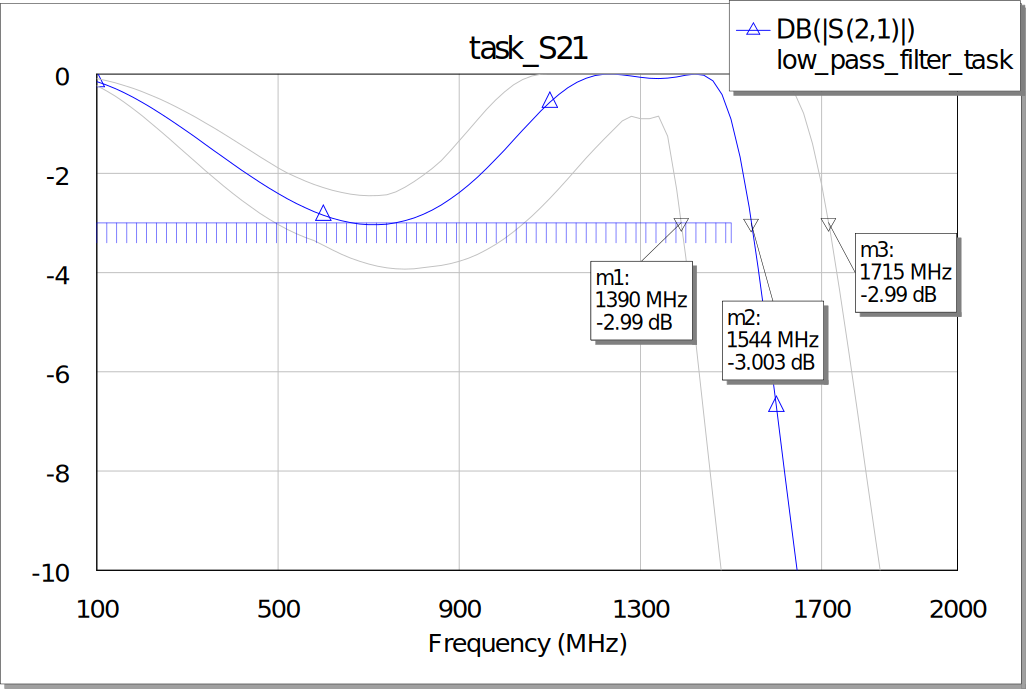
\includegraphics[width=\textwidth]{task_S21_yield_markers}
        \caption{}%
        \label{fig:task_S21_yield_markers}
    \end{subfigure}
    \hfill
    \begin{subfigure}{0.45\textwidth}
        \centering
        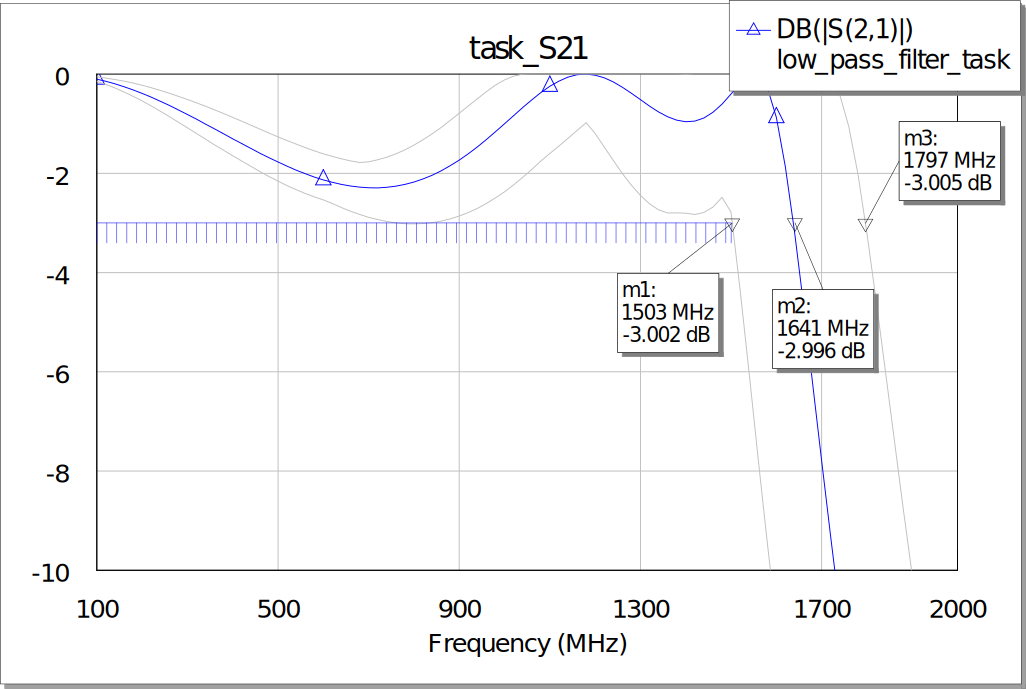
\includegraphics[width=\textwidth]{task_S21_yield_markers_modified}
        \caption{}%
        \label{fig:task_S21_yield_markers_modified}
    \end{subfigure}
    \caption{%
        (а) АЧХ проектируемого фильтра нижних частот;
        (б) АЧХ проектируемого фильтра нижних частот после установления ёмкости $C_2 = 7.8~\text{пФ}$.
    }
\end{figure}

Важно заметить, что номиналов, заданных в техническом задании, нет в рядах стандартных номиналах компонентов, что стоит учитывать, в случае, если изготавливать фильтр планируется из выводных компонентов.
